\documentclass[11pt,a4paper]{article}
\usepackage[margin=2.4cm]{geometry}
\usepackage[T1]{fontenc}
\usepackage[utf8]{inputenc}
\usepackage{lmodern}
\usepackage{microtype}
\usepackage{graphicx}
\usepackage{booktabs}
\usepackage{amsmath}
\usepackage{hyperref}
\usepackage{caption}
\usepackage{enumitem}
\usepackage{setspace}
\setstretch{1.08}
\hypersetup{colorlinks=true, linkcolor=black, citecolor=black, urlcolor=blue}

\title{\textbf{Can Large Language Models Reliably Formulate Traffic Planning Problems?}\\[0.4em]
\large A Solver-Verified Benchmark and Experimental Design on the Sioux Falls Network}
\author{Djoud El Hak Belkhir\\[0.2em]\small Repository: \url{https://github.com/djihad-elhak/llm-traffic-planning}}
\date{November 2026 \quad (technical report, version 1)}

\begin{document}
\maketitle

\begin{abstract}
Large language models (LLMs) are increasingly proposed as conversational front-ends to transportation planning tools, but a plausible answer is not a correct one: a planning recommendation is only useful if the underlying traffic model was formulated correctly. We study this gap on the Sioux Falls benchmark network. We contribute (i) a user-equilibrium traffic assignment solver validated against published equilibrium link flows, with a mean relative error of 0.008\% over 76 links; (ii) a benchmark of 40 natural-language planning scenarios (link closures, capacity changes, tolls, and demand changes), each paired with a solver-computed reference answer; and (iii) an experimental design comparing three conditions: direct estimation by the model, structured formulation followed by solving, and formulation with constraint checking and retries. We report the status of the implementation, including software tests and an end-to-end pipeline test with a deterministic mock model. The LLM experiments themselves have not yet been run; we state the hypotheses and the analysis plan in advance and describe the limitations that will bound any conclusion.
\end{abstract}

\section{Introduction}
Transportation planning relies on traffic assignment models that predict how travellers distribute themselves over a network once a change is made, such as closing a road, adding capacity, or introducing a toll. Using these models requires specialist knowledge of network formulation, cost functions, and optimization. Recent work proposes large language models as an interface that lets non-specialists express a planning question in plain language and receive an answer grounded in a model \cite{lee2026}. The appeal is clear, but the central risk is less visible: an LLM can produce a fluent, confident estimate of the effect of an intervention that does not correspond to any correct formulation of the problem.

This report addresses one narrow version of that risk. Given a plain-English planning request on a benchmark network, can an LLM identify the intervention correctly, and does adding a verification step change how often it does so? We separate two failure modes. The first is \emph{estimation failure}, where the model is asked directly for a quantitative answer and gives a number unrelated to the true outcome. The second is \emph{formulation failure}, where the model selects the wrong link, operation, or magnitude when translating the request into a model. Separating them lets us attribute errors to the step where they occur.

Our contributions are: a validated reference solver; a verifiable benchmark of 40 scenarios with reference answers; a three-condition experimental design with pre-stated hypotheses and an analysis plan; and an open, reproducible implementation. We do not claim results for the LLM conditions in this version.

\section{Related Work}
Several recent studies combine LLMs with transportation models. Lee couples an LLM, a model-context-protocol interface, the open-source AequilibraE engine, and a differentiable user-equilibrium layer, so that a planner can interact with a traffic model in natural language \cite{lee2026}. A survey of LLM agents for urban systems groups transportation applications into infrastructure optimization and human-centred services, and notes systems in which LLMs act as interfaces to traffic datasets and simulators \cite{urban2025}. Work on traffic incident management compares a hybrid approach, in which an LLM translates an event description into a structured input for an optimization algorithm and back, with a fully LLM-driven approach; the authors report that the hybrid is more reliable in high-stakes settings \cite{incident2025}. Surveys of LLMs in intelligent transportation systems describe their potential for planning and decision support \cite{its2025}.

These studies establish feasibility and, in the hybrid case, the value of solver-based verification. Our contribution is to measure formulation reliability systematically on a fixed benchmark with solver-computed references, and to separate estimation from formulation errors. The hybrid design in \cite{incident2025} motivates our condition~C; our benchmark supplies the controlled, checkable scenarios that such a comparison requires.

\section{Problem Formulation}
\subsection{Network and demand}
We use the Sioux Falls network from the Transportation Networks for Research repository \cite{tntp}: 24 nodes, 76 directed links, 528 origin--destination (OD) pairs, and a total demand of 360{,}600 trips.

\subsection{User equilibrium}
We model route choice with static user equilibrium (UE), in which no traveller can reduce their own travel time by changing route. Link travel times follow the Bureau of Public Roads (BPR) function
\begin{equation}
t_a(v_a) = t^0_a \left(1 + \alpha \left(\frac{v_a}{c_a}\right)^{\beta}\right),
\end{equation}
with free-flow time $t^0_a$, capacity $c_a$, and the network's parameters $\alpha = 0.15$ and $\beta = 4$. UE is the solution of the Beckmann program, a convex minimization whose objective is the sum of the integrals of link costs \cite{beckmann1956}. Total system travel time (TSTT), $\sum_a t_a(v_a)\, v_a$, is the primary outcome we report.

\section{Reference Solver}
\subsection{Method}
We solve UE with the Frank--Wolfe algorithm \cite{frankwolfe1956}. At each iteration, all-or-nothing assignment along shortest paths gives an auxiliary solution; the step size is found by bisection on the directional derivative of the objective to high precision. Convergence is measured by the relative gap between the total travel time under current flows and under the auxiliary assignment. Shortest paths use Dijkstra's algorithm from each zone. The implementation has no dependency beyond NumPy and SciPy.

\subsection{Validation}
We validate against the published equilibrium link flows for the same network and demand. Figure~\ref{fig:validation} compares the two across all 76 links. The mean relative error is 0.008\% and the maximum is 0.041\%. The relative gap after 5{,}000 iterations is $2.9\times10^{-5}$.

We do not validate the absolute TSTT against a published figure. Its scale depends on conventions, such as units and whether demand is expressed per hour or per day, that we have not confirmed against a reference; we therefore use TSTT only for relative comparisons within this study. Because every scenario is compared with the same baseline solved by the same code, this does not affect the relative results reported below.

\begin{figure}[t]
\centering
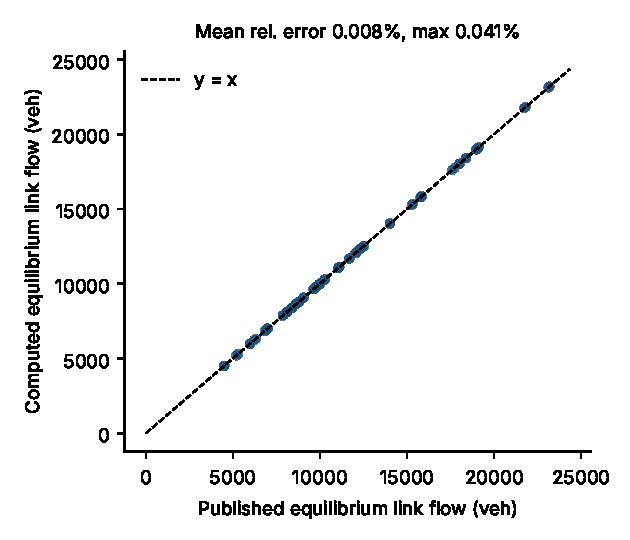
\includegraphics[width=0.55\linewidth]{fig_validation.pdf}
\caption{Computed versus published equilibrium link flows for the Sioux Falls network (76 links). The dashed line marks perfect agreement.}
\label{fig:validation}
\end{figure}

\section{Benchmark}
\subsection{Scenario generation}
Each scenario consists of a plain-English request and a machine-checkable specification of the intervention. There are four operations. \emph{Close link} removes a directed link. \emph{Capacity} multiplies a link's capacity by 1.5 or 2. \emph{Toll} adds a monetary cost to a link for route choice, excluded from TSTT. \emph{Demand} scales all OD demand by 0.9, 1.1, or 1.2. Links for closures are sampled at random and kept only if every OD pair remains reachable; the generator uses a fixed random seed (7) so the benchmark is reproducible.

Each scenario is solved once to give a reference answer. The reference is the change in TSTT relative to the baseline equilibrium.

\subsection{Distribution of outcomes}
Table~\ref{tab:bench} summarizes the 40 scenarios. The results are plausible in direction: closures and demand increases raise total travel time, and capacity increases reduce it or leave it almost unchanged. Two results are worth noting. First, a demand reduction of 10\% lowered TSTT by 25.5\%, which reflects the convexity of the BPR function rather than an error. Second, some tolls increased TSTT: travellers avoiding a tolled link can end up on longer routes, which raises total travel time, and TSTT measures travel time rather than monetary cost. The distribution of changes is shown in Figure~\ref{fig:benchmark}.

\begin{table}[t]
\centering
\caption{Benchmark scenarios and solver-computed change in total system travel time (TSTT), in percent of baseline.}
\label{tab:bench}
\begin{tabular}{lrrrr}
\toprule
Operation & $n$ & Min & Median & Max \\
\midrule
Close link & 8 & 3.23 & 9.98 & 35.92 \\
Capacity & 14 & $-3.17$ & $-0.92$ & $-0.00$ \\
Toll & 14 & $-0.11$ & 0.79 & 5.43 \\
Demand & 4 & $-25.50$ & 4.06 & 33.61 \\
\midrule
All & 40 & $-25.50$ & 0.25 & 35.92 \\
\bottomrule
\end{tabular}
\end{table}

\begin{figure}[t]
\centering
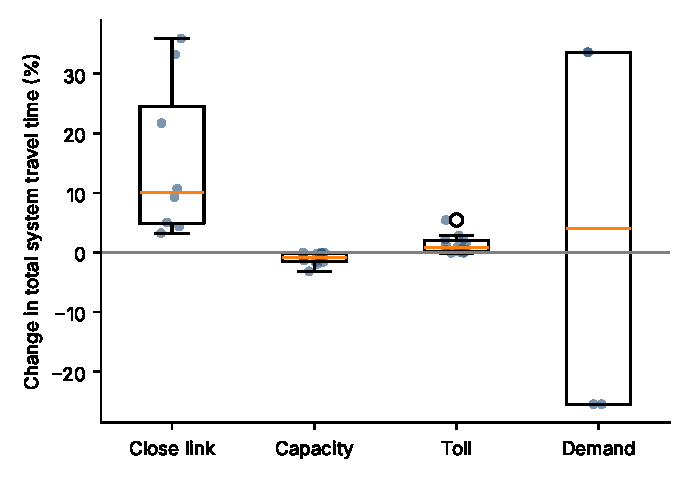
\includegraphics[width=0.6\linewidth]{fig_benchmark.pdf}
\caption{Change in TSTT by intervention type across the 40 benchmark scenarios. Points are individual scenarios, jittered horizontally.}
\label{fig:benchmark}
\end{figure}

\section{Experimental Conditions}
The model receives the request and, in conditions B and C, must output a JSON specification with an operation, a link (initial and terminal node), and a magnitude. The specification is restricted to the four operations so that its correctness can be checked against the reference. This is a deliberate simplification: the model chooses the intervention, and the solver does the optimization, so the experiment isolates formulation from solver code-writing.

\begin{description}[leftmargin=1.5em,style=nextline]
\item[Condition A (direct).] The model estimates the resulting TSTT without any solver.
\item[Condition B (formulate).] The model outputs a specification; the solver computes TSTT. Invalid specifications are not checked and produce no prediction.
\item[Condition C (verify).] As B, but each specification is checked before solving: the link must exist, the magnitude must be numeric, and closures must preserve reachability. Failed checks return the error to the model, which may retry up to two times.
\end{description}

\section{Evaluation Plan}
For each condition we will report four quantities, computed on all 40 scenarios:
\begin{enumerate}[leftmargin=1.5em]
\item \textbf{Formulation accuracy} (conditions B and C): the fraction of scenarios whose specification matches the reference operation, link, and magnitude. We report a 95\% bootstrap confidence interval from 2{,}000 resamples.
\item \textbf{TSTT error}: the relative difference between predicted and reference TSTT, reported as median and 90th percentile over scenarios with a prediction.
\item \textbf{No-prediction count}: scenarios for which no usable number was produced. This is reported separately so that failures are not hidden by the error statistics.
\item \textbf{Attempts}: the mean number of model calls per scenario, which measures the cost of verification.
\end{enumerate}

\subsection{Pre-stated hypotheses}
\begin{itemize}[leftmargin=1.5em]
\item \textbf{H1.} Condition A yields substantially larger TSTT errors than conditions B and C, because the model must reason about a network it does not compute.
\item \textbf{H2.} Condition C has higher formulation accuracy than condition B, because checking catches invalid links and magnitudes that retries can correct.
\item \textbf{H3.} Formulation accuracy is lower for closures and tolls than for capacity and demand changes, because these require selecting specific links and reasoning about routing consequences.
\end{itemize}
We will report the outcome of each hypothesis whether or not it is supported.

\subsection{Models}
The primary model is an open-weight instruction-tuned model (Qwen2.5-7B-Instruct) run in 4-bit precision on two NVIDIA T4 GPUs, so that the experiment is reproducible without paid API access. A larger model (Qwen2.5-14B-Instruct) is a planned secondary comparison, which would test whether formulation accuracy depends on model scale.

\section{Implementation and Verification of the Pipeline}
\subsection{Software}
The code is in a public repository, with a reference solver, benchmark generator, LLM harness, Streamlit demonstration, and a Kaggle notebook that runs the full experiment. Unit tests (10) cover the network loader, the BPR function, JSON parsing, the specification validator, and the equilibrium solver.

\subsection{Pipeline test with a mock model}
Before running a real model, we tested the notebook end to end with a deterministic mock model. The mock returns the correct specification on the first attempt for even-numbered scenarios and an invalid link for odd-numbered scenarios. Its purpose is to test the plumbing and the statistics, not model quality.

The test ran all 120 trials without error. Condition B produced 20 correct specifications and 20 incorrect ones; every incorrect specification named a non-existent link and therefore produced no prediction, which the no-prediction count records. Condition C recovered all 20 first-attempt errors on retry, with a mean of 1.5 attempts per scenario. The mock results are a software test only and are not evidence about any language model.

\subsection{Deployed demonstration}
A Streamlit application runs the solver interactively. Its baseline TSTT matches the value computed in our validation run, and a test intervention on a single link returned a change of +3.25\% in TSTT with a relative gap of $2.5\times10^{-5}$. The demonstration is a convenience for inspection and is not part of the evaluation.

\section{Limitations}
We list the limitations that bound the conclusions we can draw from the planned experiment.
\begin{itemize}[leftmargin=1.5em]
\item \textbf{Structured specification, not free-form models.} Conditions B and C ask the model to choose an intervention, not to write an optimization model. Results therefore speak to formulation of the intervention, not to general modelling ability.
\item \textbf{One network and one assignment model.} Results may not generalize to larger networks, dynamic assignment, or multimodal systems.
\item \textbf{Absolute TSTT not validated.} We use TSTT for relative comparisons only.
\item \textbf{Small benchmark.} Forty scenarios support descriptive comparisons with wide confidence intervals; they do not support fine-grained claims.
\item \textbf{Model scale.} The primary model is small. A low formulation accuracy would reflect this as well as the difficulty of the task, and we will report both models where possible.
\item \textbf{Scenario phrasing.} Requests are generated from templates and are stylistically uniform. Real planners write more varied requests, which may be harder to formulate.
\end{itemize}

\section{Status and Next Steps}
Completed: the reference solver and its validation; the 40-scenario benchmark with reference answers; the experimental harness; unit tests; the end-to-end pipeline test; and the deployed demonstration.

Not yet completed: running conditions A, B, and C with the open model; the secondary model; the analysis of results and confidence intervals; and the containerized service and experiment tracking.

\section{Conclusion}
We have built and validated the measurement instrument needed to test whether language models can formulate traffic planning problems reliably: a solver that matches published equilibrium flows, a benchmark whose reference answers are computed rather than assumed, and an experimental design that separates estimation from formulation. The central empirical question remains open. The experiment is designed so that its answer, whatever it is, can be attributed to a specific failure mode and reproduced from the public repository.

\begin{thebibliography}{99}
\bibitem{lee2026} Lee, E.\ (2026). Large language model assisted transportation planning through a differentiable user equilibrium layer. arXiv:2610.16140.
\bibitem{urban2025} Large language model powered intelligent urban agents: concepts, capabilities, and applications. arXiv:2507.00914.
\bibitem{incident2025} Automating the loop in traffic incident management on highway. arXiv:2503.12085.
\bibitem{its2025} Integrating LLMs with ITS: recent advances, potentials, challenges, and future directions. arXiv:2501.04437.
\bibitem{tntp} Transportation Networks for Research. \url{https://github.com/bstabler/TransportationNetworks} (Sioux Falls network, trip table, and reference flows).
\bibitem{beckmann1956} Beckmann, M., McGuire, C.\ B., \& Winsten, C.\ B.\ (1956). \emph{Studies in the Economics of Transportation}. Yale University Press.
\bibitem{frankwolfe1956} Frank, M., \& Wolfe, P.\ (1956). An algorithm for quadratic programming. \emph{Naval Research Logistics Quarterly}, 3(1--2), 95--110.
\end{thebibliography}

\end{document}
